
\begin{frame}\frametitle{A successfull theory}
\scriptsize\centering

\begin{minipage}{.55\textwidth}\centering


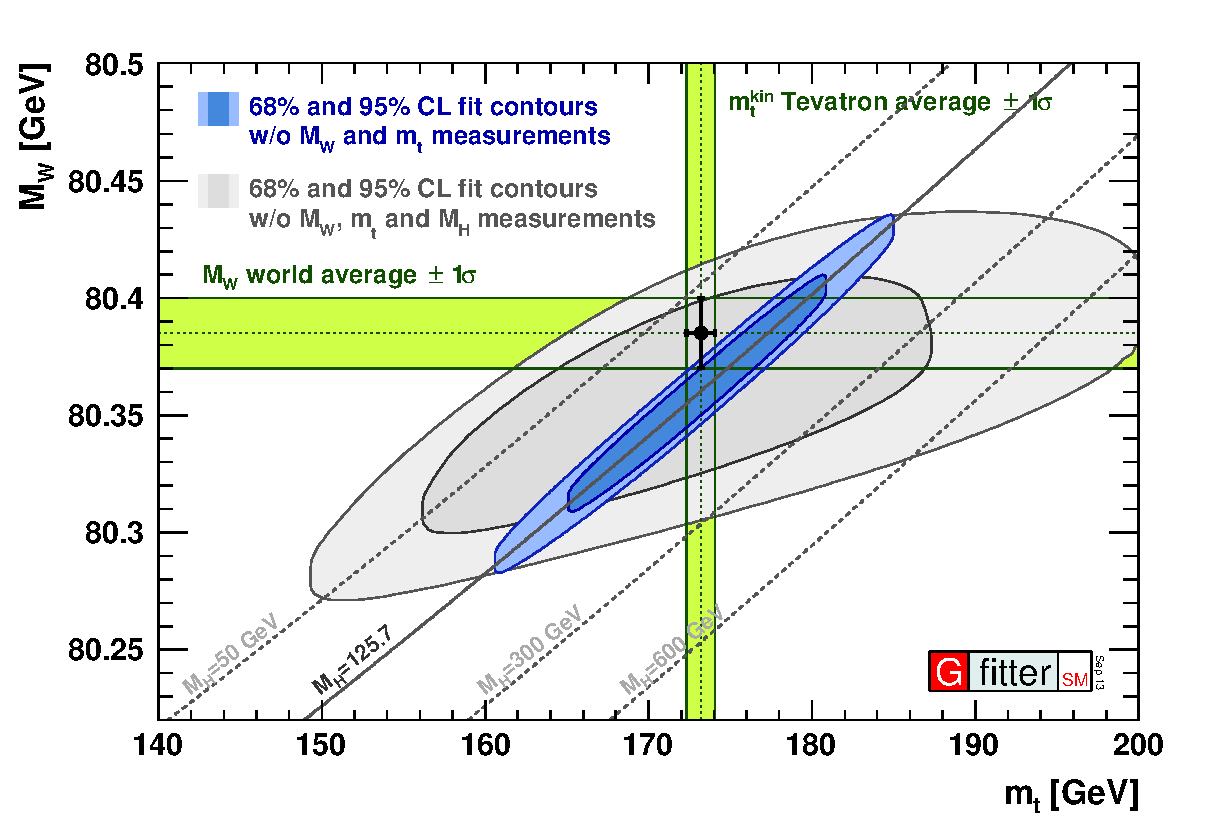
\includegraphics[width=0.8\textwidth]{pics/W_vs_top}

\resizebox{1.\textwidth}{!}{\tiny
\begin{tabular}{c x{.15\textwidth} x{.15\textwidth} x{.15\textwidth} x{.15\textwidth}}\toprule
           & \multicolumn{2}{c}{Leptons}&\multicolumn{2}{c}{Quarks} \\ 
Fermion    & \multicolumn{2}{c}{spin 1/2}& \multicolumn{2}{c}{spin 1/2}\\
generation & $q=-1$ & $q=0$ &$q=2/3$ &$q=-1/3$ \\ \midrule
I & $e^{-}$ & $\nu_{e}$ & $u$ & $d$ \\
II & $\mu^{-}$ & $\nu_{\mu}$ & $c$ & $s$ \\
III & $\tau^{-}$ & $\nu_{\tau}$ & $t$ & $b$ \\ \midrule%\bottomrule\toprule
Force & Electromagnetic &\multicolumn{2}{c}{Weak}& Strong\\\midrule
Carrier boson & $\gamma$ & $W^{\pm}$ &$Z$ & $g$\\
spin & 1 & 1 &  1 & 1 \\
$q$ & 0 & $\pm$1 & 0 & 0\\ \midrule%\bottomrule\toprule
 \multicolumn{2}{c}{Higgs boson $H$}& \multicolumn{3}{c}{$q=0$, spin=0} \\
\bottomrule
\end{tabular}
}


\end{minipage}\begin{minipage}{.45\textwidth}\centering

\vskip-5ex
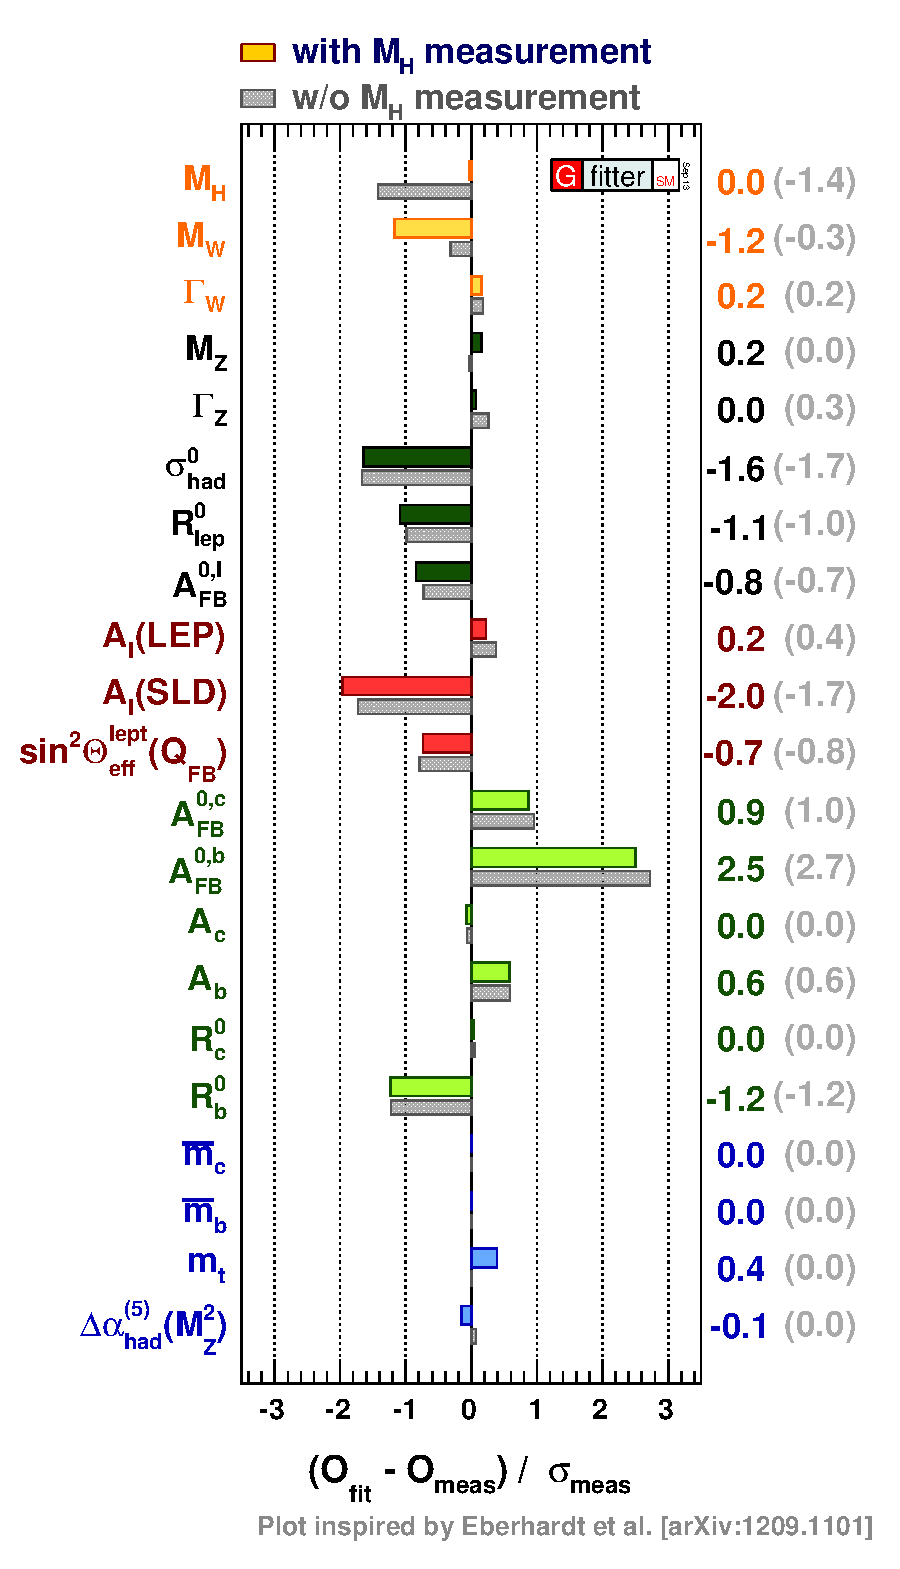
\includegraphics[width=0.8\textwidth]{pics/fitSM_new}

\end{minipage}\end{frame}


\begin{frame}\frametitle{\dots effectively}
\scriptsize\centering

\begin{pgfpicture}{0.0\textwidth}{0.0\textheight}{1.\textwidth}{.6\textwidth}

\begin{pgfscope}
\pgfdeclareimage[interpolate=true,width=.4\textwidth]{pie}{pics/piematter}
\pgfdeclareimage[interpolate=true,width=.42\textwidth]{gut}{pics/gut}
\pgfdeclareimage[interpolate=true,width=.3\textwidth]{loop}{pics/loop1}
\onslide<1->{
   \begin{pgftranslate}{\pgfpoint{0.\textwidth}{0.\textheight}}
%%%%%%%% QUARKS
{\usebeamercolor[bg]{head/foot boxes}\pgfcircle[fill]{\pgfxy(1.0,6.5)}{10pt}}
\pgfputat{\pgfxy(0.85,6.4)}{\pgfbox[left,base]{\large$u$}}
{\usebeamercolor[bg]{head/foot boxes}\pgfcircle[fill]{\pgfxy(2.0,6.5)}{10pt}}
\pgfputat{\pgfxy(1.85,6.4)}{\pgfbox[left,base]{\large$c$}}
{\usebeamercolor[bg]{head/foot boxes}\pgfcircle[fill]{\pgfxy(3.0,6.5)}{10pt}}
\pgfputat{\pgfxy(2.85,6.4)}{\pgfbox[left,base]{\large$t$}}
{\usebeamercolor[bg]{head/foot boxes}\pgfcircle[fill]{\pgfxy(1.0,5.5)}{10pt}}
\pgfputat{\pgfxy(0.85,5.4)}{\pgfbox[left,base]{\large$d$}}
{\usebeamercolor[bg]{head/foot boxes}\pgfcircle[fill]{\pgfxy(2.0,5.5)}{10pt}}
\pgfputat{\pgfxy(1.85,5.4)}{\pgfbox[left,base]{\large$s$}}
{\usebeamercolor[bg]{head/foot boxes}\pgfcircle[fill]{\pgfxy(3.0,5.5)}{10pt}}
\pgfputat{\pgfxy(2.85,5.4)}{\pgfbox[left,base]{\large$b$}}
%%%%%%%%%%% LEPTONS
{\usebeamercolor[bg]{head/foot boxes}\pgfcircle[fill]{\pgfxy(1.0,4.5)}{10pt}}
\pgfputat{\pgfxy(0.85,4.4)}{\pgfbox[left,base]{\large$e$}}
{\usebeamercolor[bg]{head/foot boxes}\pgfcircle[fill]{\pgfxy(2.0,4.5)}{10pt}}
\pgfputat{\pgfxy(1.85,4.4)}{\pgfbox[left,base]{\large$\mu$}}
{\usebeamercolor[bg]{head/foot boxes}\pgfcircle[fill]{\pgfxy(3.0,4.5)}{10pt}}
\pgfputat{\pgfxy(2.85,4.4)}{\pgfbox[left,base]{\large$\tau$}}
{\usebeamercolor[bg]{head/foot boxes}\pgfcircle[fill]{\pgfxy(1.0,3.5)}{10pt}}
\pgfputat{\pgfxy(0.85,3.4)}{\pgfbox[left,base]{\large$\nu_{e}$}}
{\usebeamercolor[bg]{head/foot boxes}\pgfcircle[fill]{\pgfxy(2.0,3.5)}{10pt}}
\pgfputat{\pgfxy(1.85,3.4)}{\pgfbox[left,base]{\large$\nu_{\mu}$}}
{\usebeamercolor[bg]{head/foot boxes}\pgfcircle[fill]{\pgfxy(3.0,3.5)}{10pt}}
\pgfputat{\pgfxy(2.85,3.4)}{\pgfbox[left,base]{\large$\nu_{\tau}$}}

%%%%%%%%%%%% WHY
{ \pgfsetlinewidth{1.pt}
  \usebeamercolor[fg]{head/foot boxes}
  \pgfrect[stroke]{\pgfxy(3.6,3.)}{\pgfxy(2.7,4)}
  \usebeamercolor[fg]{normal text}
  \pgfputat{\pgfxy(3.6,5.)}{\pgfbox[left,base]{\small\begin{tabular}{c} why only\\ 3 generations?\\ \\QCD limit:\\ 9 flavors\\ EW precision:\\ 3 neutrinos\\w/ $m_{\nu\nu}<m_Z$\end{tabular}}}
}
   \end{pgftranslate}
}
\onslide<2->{
\pgfputat{\pgfxy(7.,3.6)}{\pgfbox[left,base]{\pgfuseimage{pie}}}
}
\onslide<3->{
   \begin{pgftranslate}{\pgfpoint{0.5\textwidth}{0.05\textheight}}
\pgfputat{\pgfxy(1.5,0.1)}{\pgfbox[left,base]{\pgfuseimage{loop}}}
\pgfputat{\pgfxy(1.5,2.1)}{\pgfbox[left,base]{\small \begin{tabular}{c}$M_{H}^{2} \sim 10^{32}\gev$\\\bf \textit{hierarchy problem}\\\end{tabular}}}
\pgfputat{\pgfxy(1.7,0.4)}{\pgfbox[left,base]{\small $H \qquad\qquad t \qquad\qquad H$ }}
   \end{pgftranslate}
}
\onslide<4->{
\pgfputat{\pgfxy(0.5,0.1)}{\pgfbox[left,base]{\pgfuseimage{gut}}}
\pgfputat{\pgfxy(3.,2.1)}{\pgfbox[left,base]{\small \cccolor GUT theories? Gravity?}}
}

\end{pgfscope}
\end{pgfpicture}



\end{frame}


\begin{frame}\frametitle{Go Beyond!}
\scriptsize\centering

\begin{pgfpicture}{0.0\textwidth}{0.0\textheight}{1.\textwidth}{.6\textwidth}

\begin{pgfscope}
\pgfdeclareimage[interpolate=true,width=.28\textwidth]{kk}{pics/extradimension.pdf}
\pgfdeclareimage[interpolate=true,width=.28\textwidth]{ed}{../theory/figures/I15-71-warpedi.jpg}
\pgfdeclareimage[interpolate=true,width=.6\textwidth]{compo}{../theory/figures/compHiggs.png}
\onslide<1->{
   \begin{pgftranslate}{\pgfpoint{0.01\textwidth}{0.\textheight}}
     %%%%%%%% QUARKS
{\usebeamercolor[bg]{head/foot boxes}\pgfcircle[fill]{\pgfxy(1.0,6.5)}{10pt}}
\pgfputat{\pgfxy(0.85,6.4)}{\pgfbox[left,base]{\large$u$}}
{\usebeamercolor[bg]{head/foot boxes}\pgfcircle[fill]{\pgfxy(2.0,6.5)}{10pt}}
\pgfputat{\pgfxy(1.85,6.4)}{\pgfbox[left,base]{\large$c$}}
{\usebeamercolor[bg]{head/foot boxes}\pgfcircle[fill]{\pgfxy(3.0,6.5)}{10pt}}
\pgfputat{\pgfxy(2.85,6.4)}{\pgfbox[left,base]{\large$t$}}
{\usebeamercolor[bg]{head/foot boxes}\pgfcircle[fill]{\pgfxy(1.0,5.5)}{10pt}}
\pgfputat{\pgfxy(0.85,5.4)}{\pgfbox[left,base]{\large$d$}}
{\usebeamercolor[bg]{head/foot boxes}\pgfcircle[fill]{\pgfxy(2.0,5.5)}{10pt}}
\pgfputat{\pgfxy(1.85,5.4)}{\pgfbox[left,base]{\large$s$}}
{\usebeamercolor[bg]{head/foot boxes}\pgfcircle[fill]{\pgfxy(3.0,5.5)}{10pt}}
\pgfputat{\pgfxy(2.85,5.4)}{\pgfbox[left,base]{\large$b$}}
%%%%%%%%%%% LEPTONS
{\usebeamercolor[bg]{head/foot boxes}\pgfcircle[fill]{\pgfxy(1.0,4.5)}{10pt}}
\pgfputat{\pgfxy(0.85,4.4)}{\pgfbox[left,base]{\large$e$}}
{\usebeamercolor[bg]{head/foot boxes}\pgfcircle[fill]{\pgfxy(2.0,4.5)}{10pt}}
\pgfputat{\pgfxy(1.85,4.4)}{\pgfbox[left,base]{\large$\mu$}}
{\usebeamercolor[bg]{head/foot boxes}\pgfcircle[fill]{\pgfxy(3.0,4.5)}{10pt}}
\pgfputat{\pgfxy(2.85,4.4)}{\pgfbox[left,base]{\large$\tau$}}
{\usebeamercolor[bg]{head/foot boxes}\pgfcircle[fill]{\pgfxy(1.0,3.5)}{10pt}}
\pgfputat{\pgfxy(0.85,3.4)}{\pgfbox[left,base]{\large$\nu_{e}$}}
{\usebeamercolor[bg]{head/foot boxes}\pgfcircle[fill]{\pgfxy(2.0,3.5)}{10pt}}
\pgfputat{\pgfxy(1.85,3.4)}{\pgfbox[left,base]{\large$\nu_{\mu}$}}
{\usebeamercolor[bg]{head/foot boxes}\pgfcircle[fill]{\pgfxy(3.0,3.5)}{10pt}}
\pgfputat{\pgfxy(2.85,3.4)}{\pgfbox[left,base]{\large$\nu_{\tau}$}}

{\usebeamercolor[bg]{head/foot boxes}\pgfcircle[fill]{\pgfxy(4.0,6.5)}{10pt}}
\pgfputat{\pgfxy(3.85,6.4)}{\pgfbox[left,base]{\large$t'$}}
{\usebeamercolor[bg]{head/foot boxes}\pgfcircle[fill]{\pgfxy(4.0,5.5)}{10pt}}
\pgfputat{\pgfxy(3.85,5.4)}{\pgfbox[left,base]{\large$b'$}}
%%%%%%%%%%% LEPTONS
{\usebeamercolor[bg]{head/foot boxes}\pgfcircle[fill]{\pgfxy(4.0,4.5)}{10pt}}
\pgfputat{\pgfxy(3.85,4.4)}{\pgfbox[left,base]{\large$\tau'$}}
{\usebeamercolor[bg]{head/foot boxes}\pgfcircle[fill]{\pgfxy(4.0,3.5)}{10pt}}
\pgfputat{\pgfxy(3.85,3.4)}{\pgfbox[left,base]{\large$\nu_{\tau'}$}}

     \pgfputat{\pgfxy(-0.1,5.)}{\pgfbox[left,base]{\small \cccolor \bf SM4}}
   \end{pgftranslate}
}
\onslide<2->{
\pgfputat{\pgfxy(8.3,5.)}{\pgfbox[left,base]{\pgfuseimage{ed}}}
\pgfputat{\pgfxy(8.3,0.)}{\pgfbox[left,base]{\pgfuseimage{kk}}}
}
\onslide<3->{
\pgfputat{\pgfxy(0.5,0.1)}{\pgfbox[left,base]{\pgfuseimage{compo}}}
\pgfputat{\pgfxy(3.,2.1)}{\pgfbox[left,base]{\small \cccolor Composite Higgs}}
}
\onslide<4->{
\pgfputat{\pgfxy(5.3,4.8)}{\pgfbox[left,base]{\large \begin{tabular}{|c|} \toprule All\\ featuring\\ \bf \cccolor heavy\\ 
\bf \cccolor top\\ 
\bf \cccolor partner\\\bottomrule \end{tabular}}}
}



\end{pgfscope}
\end{pgfpicture}

\end{frame}

